% Created by tikzDevice version 0.12.6 on 2026-07-09 15:42:27
% !TEX encoding = UTF-8 Unicode
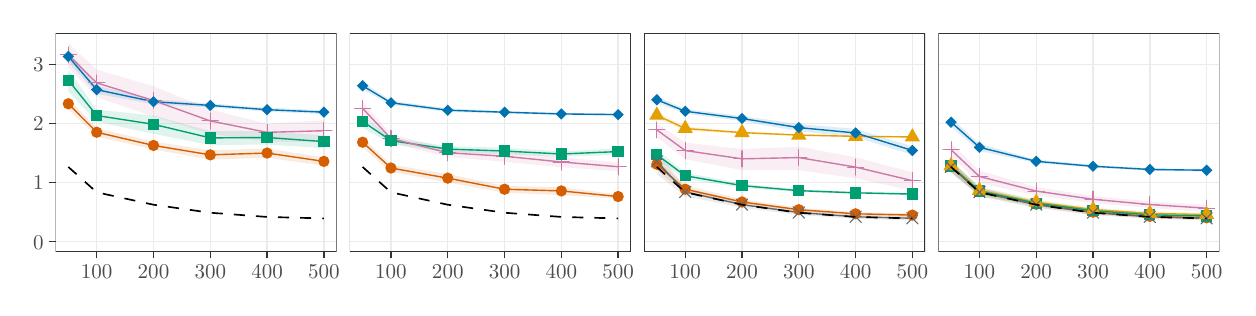
\begin{tikzpicture}[x=1pt,y=1pt]
\definecolor{fillColor}{RGB}{255,255,255}
\path[use as bounding box,fill=fillColor,fill opacity=0.00] (0,0) rectangle (433.62, 93.95);
\begin{scope}
\path[clip] (  0.00,  0.00) rectangle (433.62, 93.95);
\definecolor{drawColor}{RGB}{255,255,255}
\definecolor{fillColor}{RGB}{255,255,255}

\path[draw=drawColor,line width= 0.5pt,line join=round,line cap=round,fill=fillColor] ( -0.00,  0.00) rectangle (433.62, 93.95);
\end{scope}
\begin{scope}
\path[clip] ( 10.07, 12.99) rectangle (111.65, 91.95);
\definecolor{fillColor}{RGB}{255,255,255}

\path[fill=fillColor] ( 10.07, 12.99) rectangle (111.65, 91.95);
\definecolor{drawColor}{gray}{0.92}

\path[draw=drawColor,line width= 0.5pt,line join=round] ( 10.07, 16.58) --
	(111.65, 16.58);

\path[draw=drawColor,line width= 0.5pt,line join=round] ( 10.07, 37.94) --
	(111.65, 37.94);

\path[draw=drawColor,line width= 0.5pt,line join=round] ( 10.07, 59.29) --
	(111.65, 59.29);

\path[draw=drawColor,line width= 0.5pt,line join=round] ( 10.07, 80.65) --
	(111.65, 80.65);

\path[draw=drawColor,line width= 0.5pt,line join=round] ( 24.95, 12.99) --
	( 24.95, 91.95);

\path[draw=drawColor,line width= 0.5pt,line join=round] ( 45.47, 12.99) --
	( 45.47, 91.95);

\path[draw=drawColor,line width= 0.5pt,line join=round] ( 65.99, 12.99) --
	( 65.99, 91.95);

\path[draw=drawColor,line width= 0.5pt,line join=round] ( 86.51, 12.99) --
	( 86.51, 91.95);

\path[draw=drawColor,line width= 0.5pt,line join=round] (107.03, 12.99) --
	(107.03, 91.95);
\definecolor{fillColor}{RGB}{213,94,0}

\path[fill=fillColor,fill opacity=0.12] ( 14.69, 68.33) --
	( 24.95, 57.64) --
	( 45.47, 52.76) --
	( 65.99, 49.64) --
	( 86.51, 50.26) --
	(107.03, 47.09) --
	(107.03, 44.10) --
	( 86.51, 46.96) --
	( 65.99, 46.26) --
	( 45.47, 49.97) --
	( 24.95, 54.62) --
	( 14.69, 64.49) --
	cycle;

\path[] ( 14.69, 68.33) --
	( 24.95, 57.64) --
	( 45.47, 52.76) --
	( 65.99, 49.64) --
	( 86.51, 50.26) --
	(107.03, 47.09);

\path[] (107.03, 44.10) --
	( 86.51, 46.96) --
	( 65.99, 46.26) --
	( 45.47, 49.97) --
	( 24.95, 54.62) --
	( 14.69, 64.49);
\definecolor{fillColor}{RGB}{0,158,115}

\path[fill=fillColor,fill opacity=0.12] ( 14.69, 78.80) --
	( 24.95, 64.31) --
	( 45.47, 62.21) --
	( 65.99, 56.56) --
	( 86.51, 56.62) --
	(107.03, 54.99) --
	(107.03, 50.43) --
	( 86.51, 51.73) --
	( 65.99, 51.51) --
	( 45.47, 55.60) --
	( 24.95, 59.99) --
	( 14.69, 70.87) --
	cycle;

\path[] ( 14.69, 78.80) --
	( 24.95, 64.31) --
	( 45.47, 62.21) --
	( 65.99, 56.56) --
	( 86.51, 56.62) --
	(107.03, 54.99);

\path[] (107.03, 50.43) --
	( 86.51, 51.73) --
	( 65.99, 51.51) --
	( 45.47, 55.60) --
	( 24.95, 59.99) --
	( 14.69, 70.87);
\definecolor{fillColor}{RGB}{0,114,178}

\path[fill=fillColor,fill opacity=0.12] ( 14.69, 85.46) --
	( 24.95, 73.00) --
	( 45.47, 68.11) --
	( 65.99, 66.58) --
	( 86.51, 65.02) --
	(107.03, 64.11) --
	(107.03, 62.71) --
	( 86.51, 63.59) --
	( 65.99, 65.13) --
	( 45.47, 66.27) --
	( 24.95, 70.06) --
	( 14.69, 81.60) --
	cycle;

\path[] ( 14.69, 85.46) --
	( 24.95, 73.00) --
	( 45.47, 68.11) --
	( 65.99, 66.58) --
	( 86.51, 65.02) --
	(107.03, 64.11);

\path[] (107.03, 62.71) --
	( 86.51, 63.59) --
	( 65.99, 65.13) --
	( 45.47, 66.27) --
	( 24.95, 70.06) --
	( 14.69, 81.60);
\definecolor{fillColor}{RGB}{204,121,167}

\path[fill=fillColor,fill opacity=0.12] ( 14.69, 88.36) --
	( 24.95, 78.73) --
	( 45.47, 72.81) --
	( 65.99, 64.43) --
	( 86.51, 59.20) --
	(107.03, 60.49) --
	(107.03, 52.54) --
	( 86.51, 52.79) --
	( 65.99, 55.63) --
	( 45.47, 61.83) --
	( 24.95, 68.82) --
	( 14.69, 79.58) --
	cycle;

\path[] ( 14.69, 88.36) --
	( 24.95, 78.73) --
	( 45.47, 72.81) --
	( 65.99, 64.43) --
	( 86.51, 59.20) --
	(107.03, 60.49);

\path[] (107.03, 52.54) --
	( 86.51, 52.79) --
	( 65.99, 55.63) --
	( 45.47, 61.83) --
	( 24.95, 68.82) --
	( 14.69, 79.58);
\definecolor{drawColor}{RGB}{213,94,0}

\path[draw=drawColor,line width= 0.5pt,line join=round] ( 14.69, 66.45) --
	( 24.95, 56.16) --
	( 45.47, 51.39) --
	( 65.99, 47.99) --
	( 86.51, 48.65) --
	(107.03, 45.63);
\definecolor{drawColor}{RGB}{0,158,115}

\path[draw=drawColor,line width= 0.5pt,line join=round] ( 14.69, 74.97) --
	( 24.95, 62.20) --
	( 45.47, 59.03) --
	( 65.99, 54.12) --
	( 86.51, 54.26) --
	(107.03, 52.78);
\definecolor{drawColor}{RGB}{0,114,178}

\path[draw=drawColor,line width= 0.5pt,line join=round] ( 14.69, 83.56) --
	( 24.95, 71.55) --
	( 45.47, 67.20) --
	( 65.99, 65.86) --
	( 86.51, 64.31) --
	(107.03, 63.42);
\definecolor{drawColor}{RGB}{204,121,167}

\path[draw=drawColor,line width= 0.5pt,line join=round] ( 14.69, 84.12) --
	( 24.95, 73.99) --
	( 45.47, 67.62) --
	( 65.99, 60.25) --
	( 86.51, 56.13) --
	(107.03, 56.71);
\definecolor{fillColor}{RGB}{213,94,0}

\path[fill=fillColor] ( 14.69, 66.45) circle (  2.05);

\path[draw=drawColor,line width= 0.4pt,line join=round,line cap=round] ( 11.79, 84.12) -- ( 17.59, 84.12);

\path[draw=drawColor,line width= 0.4pt,line join=round,line cap=round] ( 14.69, 81.21) -- ( 14.69, 87.02);
\definecolor{fillColor}{RGB}{0,158,115}

\path[fill=fillColor] ( 12.64, 72.92) --
	( 16.74, 72.92) --
	( 16.74, 77.02) --
	( 12.64, 77.02) --
	cycle;
\definecolor{fillColor}{RGB}{0,114,178}

\path[fill=fillColor] ( 12.64, 83.56) --
	( 14.69, 85.61) --
	( 16.74, 83.56) --
	( 14.69, 81.51) --
	cycle;
\definecolor{fillColor}{RGB}{213,94,0}

\path[fill=fillColor] ( 24.95, 56.16) circle (  2.05);

\path[draw=drawColor,line width= 0.4pt,line join=round,line cap=round] ( 22.05, 73.99) -- ( 27.85, 73.99);

\path[draw=drawColor,line width= 0.4pt,line join=round,line cap=round] ( 24.95, 71.09) -- ( 24.95, 76.89);
\definecolor{fillColor}{RGB}{0,158,115}

\path[fill=fillColor] ( 22.90, 60.15) --
	( 27.00, 60.15) --
	( 27.00, 64.25) --
	( 22.90, 64.25) --
	cycle;
\definecolor{fillColor}{RGB}{0,114,178}

\path[fill=fillColor] ( 22.90, 71.55) --
	( 24.95, 73.60) --
	( 27.00, 71.55) --
	( 24.95, 69.50) --
	cycle;
\definecolor{fillColor}{RGB}{213,94,0}

\path[fill=fillColor] ( 45.47, 51.39) circle (  2.05);

\path[draw=drawColor,line width= 0.4pt,line join=round,line cap=round] ( 42.57, 67.62) -- ( 48.37, 67.62);

\path[draw=drawColor,line width= 0.4pt,line join=round,line cap=round] ( 45.47, 64.72) -- ( 45.47, 70.52);
\definecolor{fillColor}{RGB}{0,158,115}

\path[fill=fillColor] ( 43.42, 56.98) --
	( 47.52, 56.98) --
	( 47.52, 61.09) --
	( 43.42, 61.09) --
	cycle;
\definecolor{fillColor}{RGB}{0,114,178}

\path[fill=fillColor] ( 43.42, 67.20) --
	( 45.47, 69.25) --
	( 47.52, 67.20) --
	( 45.47, 65.15) --
	cycle;
\definecolor{fillColor}{RGB}{213,94,0}

\path[fill=fillColor] ( 65.99, 47.99) circle (  2.05);

\path[draw=drawColor,line width= 0.4pt,line join=round,line cap=round] ( 63.09, 60.25) -- ( 68.89, 60.25);

\path[draw=drawColor,line width= 0.4pt,line join=round,line cap=round] ( 65.99, 57.35) -- ( 65.99, 63.15);
\definecolor{fillColor}{RGB}{0,158,115}

\path[fill=fillColor] ( 63.94, 52.07) --
	( 68.04, 52.07) --
	( 68.04, 56.17) --
	( 63.94, 56.17) --
	cycle;
\definecolor{fillColor}{RGB}{0,114,178}

\path[fill=fillColor] ( 63.94, 65.86) --
	( 65.99, 67.91) --
	( 68.04, 65.86) --
	( 65.99, 63.81) --
	cycle;
\definecolor{fillColor}{RGB}{213,94,0}

\path[fill=fillColor] ( 86.51, 48.65) circle (  2.05);

\path[draw=drawColor,line width= 0.4pt,line join=round,line cap=round] ( 83.61, 56.13) -- ( 89.41, 56.13);

\path[draw=drawColor,line width= 0.4pt,line join=round,line cap=round] ( 86.51, 53.23) -- ( 86.51, 59.03);
\definecolor{fillColor}{RGB}{0,158,115}

\path[fill=fillColor] ( 84.46, 52.21) --
	( 88.56, 52.21) --
	( 88.56, 56.31) --
	( 84.46, 56.31) --
	cycle;
\definecolor{fillColor}{RGB}{0,114,178}

\path[fill=fillColor] ( 84.46, 64.31) --
	( 86.51, 66.36) --
	( 88.56, 64.31) --
	( 86.51, 62.26) --
	cycle;
\definecolor{fillColor}{RGB}{213,94,0}

\path[fill=fillColor] (107.03, 45.63) circle (  2.05);

\path[draw=drawColor,line width= 0.4pt,line join=round,line cap=round] (104.13, 56.71) -- (109.93, 56.71);

\path[draw=drawColor,line width= 0.4pt,line join=round,line cap=round] (107.03, 53.81) -- (107.03, 59.61);
\definecolor{fillColor}{RGB}{0,158,115}

\path[fill=fillColor] (104.98, 50.73) --
	(109.08, 50.73) --
	(109.08, 54.83) --
	(104.98, 54.83) --
	cycle;
\definecolor{fillColor}{RGB}{0,114,178}

\path[fill=fillColor] (104.98, 63.42) --
	(107.03, 65.47) --
	(109.08, 63.42) --
	(107.03, 61.37) --
	cycle;
\definecolor{drawColor}{RGB}{0,0,0}

\path[draw=drawColor,line width= 0.6pt,dash pattern=on 4pt off 4pt ,line join=round] ( 14.69, 43.62) --
	( 24.95, 34.46) --
	( 45.47, 29.97) --
	( 65.99, 27.08) --
	( 86.51, 25.56) --
	(107.03, 25.02);
\definecolor{drawColor}{gray}{0.20}

\path[draw=drawColor,line width= 0.5pt,line join=round,line cap=round] ( 10.07, 12.99) rectangle (111.65, 91.95);
\end{scope}
\begin{scope}
\path[clip] (116.40, 12.99) rectangle (217.97, 91.95);
\definecolor{fillColor}{RGB}{255,255,255}

\path[fill=fillColor] (116.40, 12.99) rectangle (217.97, 91.95);
\definecolor{drawColor}{gray}{0.92}

\path[draw=drawColor,line width= 0.5pt,line join=round] (116.40, 16.58) --
	(217.97, 16.58);

\path[draw=drawColor,line width= 0.5pt,line join=round] (116.40, 37.94) --
	(217.97, 37.94);

\path[draw=drawColor,line width= 0.5pt,line join=round] (116.40, 59.29) --
	(217.97, 59.29);

\path[draw=drawColor,line width= 0.5pt,line join=round] (116.40, 80.65) --
	(217.97, 80.65);

\path[draw=drawColor,line width= 0.5pt,line join=round] (131.28, 12.99) --
	(131.28, 91.95);

\path[draw=drawColor,line width= 0.5pt,line join=round] (151.80, 12.99) --
	(151.80, 91.95);

\path[draw=drawColor,line width= 0.5pt,line join=round] (172.32, 12.99) --
	(172.32, 91.95);

\path[draw=drawColor,line width= 0.5pt,line join=round] (192.84, 12.99) --
	(192.84, 91.95);

\path[draw=drawColor,line width= 0.5pt,line join=round] (213.36, 12.99) --
	(213.36, 91.95);
\definecolor{fillColor}{RGB}{213,94,0}

\path[fill=fillColor,fill opacity=0.12] (121.02, 54.32) --
	(131.28, 44.52) --
	(151.80, 41.07) --
	(172.32, 36.75) --
	(192.84, 36.34) --
	(213.36, 33.64) --
	(213.36, 32.19) --
	(192.84, 33.47) --
	(172.32, 34.32) --
	(151.80, 37.98) --
	(131.28, 41.89) --
	(121.02, 50.72) --
	cycle;

\path[] (121.02, 54.32) --
	(131.28, 44.52) --
	(151.80, 41.07) --
	(172.32, 36.75) --
	(192.84, 36.34) --
	(213.36, 33.64);

\path[] (213.36, 32.19) --
	(192.84, 33.47) --
	(172.32, 34.32) --
	(151.80, 37.98) --
	(131.28, 41.89) --
	(121.02, 50.72);
\definecolor{fillColor}{RGB}{0,158,115}

\path[fill=fillColor,fill opacity=0.12] (121.02, 62.24) --
	(131.28, 54.24) --
	(151.80, 51.15) --
	(172.32, 50.54) --
	(192.84, 49.25) --
	(213.36, 50.31) --
	(213.36, 47.98) --
	(192.84, 47.32) --
	(172.32, 48.16) --
	(151.80, 48.97) --
	(131.28, 51.96) --
	(121.02, 57.83) --
	cycle;

\path[] (121.02, 62.24) --
	(131.28, 54.24) --
	(151.80, 51.15) --
	(172.32, 50.54) --
	(192.84, 49.25) --
	(213.36, 50.31);

\path[] (213.36, 47.98) --
	(192.84, 47.32) --
	(172.32, 48.16) --
	(151.80, 48.97) --
	(131.28, 51.96) --
	(121.02, 57.83);
\definecolor{fillColor}{RGB}{0,114,178}

\path[fill=fillColor,fill opacity=0.12] (121.02, 74.24) --
	(131.28, 67.62) --
	(151.80, 64.76) --
	(172.32, 63.86) --
	(192.84, 63.16) --
	(213.36, 62.91) --
	(213.36, 62.17) --
	(192.84, 62.39) --
	(172.32, 62.94) --
	(151.80, 63.47) --
	(131.28, 66.01) --
	(121.02, 71.65) --
	cycle;

\path[] (121.02, 74.24) --
	(131.28, 67.62) --
	(151.80, 64.76) --
	(172.32, 63.86) --
	(192.84, 63.16) --
	(213.36, 62.91);

\path[] (213.36, 62.17) --
	(192.84, 62.39) --
	(172.32, 62.94) --
	(151.80, 63.47) --
	(131.28, 66.01) --
	(121.02, 71.65);
\definecolor{fillColor}{RGB}{204,121,167}

\path[fill=fillColor,fill opacity=0.12] (121.02, 67.26) --
	(131.28, 55.44) --
	(151.80, 50.20) --
	(172.32, 49.34) --
	(192.84, 47.19) --
	(213.36, 45.21) --
	(213.36, 42.09) --
	(192.84, 43.54) --
	(172.32, 45.50) --
	(151.80, 47.23) --
	(131.28, 52.32) --
	(121.02, 62.21) --
	cycle;

\path[] (121.02, 67.26) --
	(131.28, 55.44) --
	(151.80, 50.20) --
	(172.32, 49.34) --
	(192.84, 47.19) --
	(213.36, 45.21);

\path[] (213.36, 42.09) --
	(192.84, 43.54) --
	(172.32, 45.50) --
	(151.80, 47.23) --
	(131.28, 52.32) --
	(121.02, 62.21);
\definecolor{drawColor}{RGB}{213,94,0}

\path[draw=drawColor,line width= 0.5pt,line join=round] (121.02, 52.56) --
	(131.28, 43.24) --
	(151.80, 39.57) --
	(172.32, 35.57) --
	(192.84, 34.96) --
	(213.36, 32.93);
\definecolor{drawColor}{RGB}{0,158,115}

\path[draw=drawColor,line width= 0.5pt,line join=round] (121.02, 60.09) --
	(131.28, 53.12) --
	(151.80, 50.08) --
	(172.32, 49.37) --
	(192.84, 48.30) --
	(213.36, 49.17);
\definecolor{drawColor}{RGB}{0,114,178}

\path[draw=drawColor,line width= 0.5pt,line join=round] (121.02, 72.96) --
	(131.28, 66.82) --
	(151.80, 64.12) --
	(172.32, 63.40) --
	(192.84, 62.78) --
	(213.36, 62.54);
\definecolor{drawColor}{RGB}{204,121,167}

\path[draw=drawColor,line width= 0.5pt,line join=round] (121.02, 64.80) --
	(131.28, 53.91) --
	(151.80, 48.75) --
	(172.32, 47.48) --
	(192.84, 45.42) --
	(213.36, 43.70);
\definecolor{fillColor}{RGB}{213,94,0}

\path[fill=fillColor] (121.02, 52.56) circle (  2.05);

\path[draw=drawColor,line width= 0.4pt,line join=round,line cap=round] (118.11, 64.80) -- (123.92, 64.80);

\path[draw=drawColor,line width= 0.4pt,line join=round,line cap=round] (121.02, 61.90) -- (121.02, 67.70);
\definecolor{fillColor}{RGB}{0,158,115}

\path[fill=fillColor] (118.96, 58.04) --
	(123.07, 58.04) --
	(123.07, 62.14) --
	(118.96, 62.14) --
	cycle;
\definecolor{fillColor}{RGB}{0,114,178}

\path[fill=fillColor] (118.96, 72.96) --
	(121.02, 75.01) --
	(123.07, 72.96) --
	(121.02, 70.91) --
	cycle;
\definecolor{fillColor}{RGB}{213,94,0}

\path[fill=fillColor] (131.28, 43.24) circle (  2.05);

\path[draw=drawColor,line width= 0.4pt,line join=round,line cap=round] (128.37, 53.91) -- (134.18, 53.91);

\path[draw=drawColor,line width= 0.4pt,line join=round,line cap=round] (131.28, 51.01) -- (131.28, 56.82);
\definecolor{fillColor}{RGB}{0,158,115}

\path[fill=fillColor] (129.22, 51.07) --
	(133.33, 51.07) --
	(133.33, 55.17) --
	(129.22, 55.17) --
	cycle;
\definecolor{fillColor}{RGB}{0,114,178}

\path[fill=fillColor] (129.22, 66.82) --
	(131.28, 68.87) --
	(133.33, 66.82) --
	(131.28, 64.77) --
	cycle;
\definecolor{fillColor}{RGB}{213,94,0}

\path[fill=fillColor] (151.80, 39.57) circle (  2.05);

\path[draw=drawColor,line width= 0.4pt,line join=round,line cap=round] (148.89, 48.75) -- (154.70, 48.75);

\path[draw=drawColor,line width= 0.4pt,line join=round,line cap=round] (151.80, 45.85) -- (151.80, 51.65);
\definecolor{fillColor}{RGB}{0,158,115}

\path[fill=fillColor] (149.74, 48.03) --
	(153.85, 48.03) --
	(153.85, 52.13) --
	(149.74, 52.13) --
	cycle;
\definecolor{fillColor}{RGB}{0,114,178}

\path[fill=fillColor] (149.74, 64.12) --
	(151.80, 66.17) --
	(153.85, 64.12) --
	(151.80, 62.07) --
	cycle;
\definecolor{fillColor}{RGB}{213,94,0}

\path[fill=fillColor] (172.32, 35.57) circle (  2.05);

\path[draw=drawColor,line width= 0.4pt,line join=round,line cap=round] (169.41, 47.48) -- (175.22, 47.48);

\path[draw=drawColor,line width= 0.4pt,line join=round,line cap=round] (172.32, 44.58) -- (172.32, 50.38);
\definecolor{fillColor}{RGB}{0,158,115}

\path[fill=fillColor] (170.26, 47.32) --
	(174.37, 47.32) --
	(174.37, 51.42) --
	(170.26, 51.42) --
	cycle;
\definecolor{fillColor}{RGB}{0,114,178}

\path[fill=fillColor] (170.26, 63.40) --
	(172.32, 65.45) --
	(174.37, 63.40) --
	(172.32, 61.35) --
	cycle;
\definecolor{fillColor}{RGB}{213,94,0}

\path[fill=fillColor] (192.84, 34.96) circle (  2.05);

\path[draw=drawColor,line width= 0.4pt,line join=round,line cap=round] (189.93, 45.42) -- (195.74, 45.42);

\path[draw=drawColor,line width= 0.4pt,line join=round,line cap=round] (192.84, 42.52) -- (192.84, 48.32);
\definecolor{fillColor}{RGB}{0,158,115}

\path[fill=fillColor] (190.78, 46.25) --
	(194.89, 46.25) --
	(194.89, 50.35) --
	(190.78, 50.35) --
	cycle;
\definecolor{fillColor}{RGB}{0,114,178}

\path[fill=fillColor] (190.78, 62.78) --
	(192.84, 64.83) --
	(194.89, 62.78) --
	(192.84, 60.73) --
	cycle;
\definecolor{fillColor}{RGB}{213,94,0}

\path[fill=fillColor] (213.36, 32.93) circle (  2.05);

\path[draw=drawColor,line width= 0.4pt,line join=round,line cap=round] (210.45, 43.70) -- (216.26, 43.70);

\path[draw=drawColor,line width= 0.4pt,line join=round,line cap=round] (213.36, 40.80) -- (213.36, 46.60);
\definecolor{fillColor}{RGB}{0,158,115}

\path[fill=fillColor] (211.30, 47.12) --
	(215.41, 47.12) --
	(215.41, 51.22) --
	(211.30, 51.22) --
	cycle;
\definecolor{fillColor}{RGB}{0,114,178}

\path[fill=fillColor] (211.30, 62.54) --
	(213.36, 64.60) --
	(215.41, 62.54) --
	(213.36, 60.49) --
	cycle;
\definecolor{drawColor}{RGB}{0,0,0}

\path[draw=drawColor,line width= 0.6pt,dash pattern=on 4pt off 4pt ,line join=round] (121.02, 43.62) --
	(131.28, 34.46) --
	(151.80, 29.97) --
	(172.32, 27.08) --
	(192.84, 25.56) --
	(213.36, 25.02);
\definecolor{drawColor}{gray}{0.20}

\path[draw=drawColor,line width= 0.5pt,line join=round,line cap=round] (116.40, 12.99) rectangle (217.97, 91.95);
\end{scope}
\begin{scope}
\path[clip] (222.72, 12.99) rectangle (324.30, 91.95);
\definecolor{fillColor}{RGB}{255,255,255}

\path[fill=fillColor] (222.72, 12.99) rectangle (324.30, 91.95);
\definecolor{drawColor}{gray}{0.92}

\path[draw=drawColor,line width= 0.5pt,line join=round] (222.72, 16.58) --
	(324.30, 16.58);

\path[draw=drawColor,line width= 0.5pt,line join=round] (222.72, 37.94) --
	(324.30, 37.94);

\path[draw=drawColor,line width= 0.5pt,line join=round] (222.72, 59.29) --
	(324.30, 59.29);

\path[draw=drawColor,line width= 0.5pt,line join=round] (222.72, 80.65) --
	(324.30, 80.65);

\path[draw=drawColor,line width= 0.5pt,line join=round] (237.60, 12.99) --
	(237.60, 91.95);

\path[draw=drawColor,line width= 0.5pt,line join=round] (258.12, 12.99) --
	(258.12, 91.95);

\path[draw=drawColor,line width= 0.5pt,line join=round] (278.64, 12.99) --
	(278.64, 91.95);

\path[draw=drawColor,line width= 0.5pt,line join=round] (299.16, 12.99) --
	(299.16, 91.95);

\path[draw=drawColor,line width= 0.5pt,line join=round] (319.68, 12.99) --
	(319.68, 91.95);
\definecolor{fillColor}{RGB}{213,94,0}

\path[fill=fillColor,fill opacity=0.12] (227.34, 46.54) --
	(237.60, 36.93) --
	(258.12, 31.95) --
	(278.64, 28.95) --
	(299.16, 27.29) --
	(319.68, 26.87) --
	(319.68, 25.53) --
	(299.16, 26.06) --
	(278.64, 27.36) --
	(258.12, 29.94) --
	(237.60, 34.13) --
	(227.34, 42.50) --
	cycle;

\path[] (227.34, 46.54) --
	(237.60, 36.93) --
	(258.12, 31.95) --
	(278.64, 28.95) --
	(299.16, 27.29) --
	(319.68, 26.87);

\path[] (319.68, 25.53) --
	(299.16, 26.06) --
	(278.64, 27.36) --
	(258.12, 29.94) --
	(237.60, 34.13) --
	(227.34, 42.50);
\definecolor{fillColor}{RGB}{230,159,0}

\path[fill=fillColor,fill opacity=0.12] (227.34, 63.46) --
	(237.60, 58.24) --
	(258.12, 56.43) --
	(278.64, 55.44) --
	(299.16, 54.89) --
	(319.68, 54.67) --
	(319.68, 54.27) --
	(299.16, 54.46) --
	(278.64, 54.81) --
	(258.12, 55.63) --
	(237.60, 56.76) --
	(227.34, 61.08) --
	cycle;

\path[] (227.34, 63.46) --
	(237.60, 58.24) --
	(258.12, 56.43) --
	(278.64, 55.44) --
	(299.16, 54.89) --
	(319.68, 54.67);

\path[] (319.68, 54.27) --
	(299.16, 54.46) --
	(278.64, 54.81) --
	(258.12, 55.63) --
	(237.60, 56.76) --
	(227.34, 61.08);
\definecolor{fillColor}{RGB}{0,158,115}

\path[fill=fillColor,fill opacity=0.12] (227.34, 49.85) --
	(237.60, 41.54) --
	(258.12, 37.58) --
	(278.64, 35.56) --
	(299.16, 34.68) --
	(319.68, 34.18) --
	(319.68, 33.45) --
	(299.16, 33.86) --
	(278.64, 34.53) --
	(258.12, 36.12) --
	(237.60, 39.30) --
	(227.34, 46.14) --
	cycle;

\path[] (227.34, 49.85) --
	(237.60, 41.54) --
	(258.12, 37.58) --
	(278.64, 35.56) --
	(299.16, 34.68) --
	(319.68, 34.18);

\path[] (319.68, 33.45) --
	(299.16, 33.86) --
	(278.64, 34.53) --
	(258.12, 36.12) --
	(237.60, 39.30) --
	(227.34, 46.14);
\definecolor{fillColor}{RGB}{0,114,178}

\path[fill=fillColor,fill opacity=0.12] (227.34, 69.12) --
	(237.60, 64.56) --
	(258.12, 62.04) --
	(278.64, 59.13) --
	(299.16, 57.36) --
	(319.68, 51.07) --
	(319.68, 48.03) --
	(299.16, 54.38) --
	(278.64, 56.52) --
	(258.12, 60.17) --
	(237.60, 62.91) --
	(227.34, 66.66) --
	cycle;

\path[] (227.34, 69.12) --
	(237.60, 64.56) --
	(258.12, 62.04) --
	(278.64, 59.13) --
	(299.16, 57.36) --
	(319.68, 51.07);

\path[] (319.68, 48.03) --
	(299.16, 54.38) --
	(278.64, 56.52) --
	(258.12, 60.17) --
	(237.60, 62.91) --
	(227.34, 66.66);
\definecolor{fillColor}{RGB}{204,121,167}

\path[fill=fillColor,fill opacity=0.12] (227.34, 59.41) --
	(237.60, 52.40) --
	(258.12, 50.13) --
	(278.64, 50.96) --
	(299.16, 47.10) --
	(319.68, 41.72) --
	(319.68, 35.13) --
	(299.16, 39.52) --
	(278.64, 42.47) --
	(258.12, 42.48) --
	(237.60, 46.42) --
	(227.34, 54.46) --
	cycle;

\path[] (227.34, 59.41) --
	(237.60, 52.40) --
	(258.12, 50.13) --
	(278.64, 50.96) --
	(299.16, 47.10) --
	(319.68, 41.72);

\path[] (319.68, 35.13) --
	(299.16, 39.52) --
	(278.64, 42.47) --
	(258.12, 42.48) --
	(237.60, 46.42) --
	(227.34, 54.46);
\definecolor{fillColor}{RGB}{102,102,102}

\path[fill=fillColor,fill opacity=0.12] (227.34, 49.59) --
	(237.60, 36.05) --
	(258.12, 31.08) --
	(278.64, 27.99) --
	(299.16, 26.27) --
	(319.68, 25.81) --
	(319.68, 24.31) --
	(299.16, 24.91) --
	(278.64, 26.27) --
	(258.12, 28.86) --
	(237.60, 33.08) --
	(227.34, 41.01) --
	cycle;

\path[] (227.34, 49.59) --
	(237.60, 36.05) --
	(258.12, 31.08) --
	(278.64, 27.99) --
	(299.16, 26.27) --
	(319.68, 25.81);

\path[] (319.68, 24.31) --
	(299.16, 24.91) --
	(278.64, 26.27) --
	(258.12, 28.86) --
	(237.60, 33.08) --
	(227.34, 41.01);
\definecolor{drawColor}{RGB}{213,94,0}

\path[draw=drawColor,line width= 0.5pt,line join=round] (227.34, 44.59) --
	(237.60, 35.58) --
	(258.12, 30.98) --
	(278.64, 28.18) --
	(299.16, 26.69) --
	(319.68, 26.22);
\definecolor{drawColor}{RGB}{230,159,0}

\path[draw=drawColor,line width= 0.5pt,line join=round] (227.34, 62.29) --
	(237.60, 57.51) --
	(258.12, 56.03) --
	(278.64, 55.13) --
	(299.16, 54.68) --
	(319.68, 54.47);
\definecolor{drawColor}{RGB}{0,158,115}

\path[draw=drawColor,line width= 0.5pt,line join=round] (227.34, 48.05) --
	(237.60, 40.44) --
	(258.12, 36.87) --
	(278.64, 35.05) --
	(299.16, 34.27) --
	(319.68, 33.82);
\definecolor{drawColor}{RGB}{0,114,178}

\path[draw=drawColor,line width= 0.5pt,line join=round] (227.34, 67.90) --
	(237.60, 63.74) --
	(258.12, 61.12) --
	(278.64, 57.85) --
	(299.16, 55.90) --
	(319.68, 49.58);
\definecolor{drawColor}{RGB}{204,121,167}

\path[draw=drawColor,line width= 0.5pt,line join=round] (227.34, 57.01) --
	(237.60, 49.55) --
	(258.12, 46.55) --
	(278.64, 47.01) --
	(299.16, 43.57) --
	(319.68, 38.67);
\definecolor{drawColor}{gray}{0.40}

\path[draw=drawColor,line width= 0.5pt,line join=round] (227.34, 45.62) --
	(237.60, 34.63) --
	(258.12, 30.02) --
	(278.64, 27.16) --
	(299.16, 25.61) --
	(319.68, 25.09);
\definecolor{fillColor}{RGB}{213,94,0}

\path[fill=fillColor] (227.34, 44.59) circle (  2.05);
\definecolor{drawColor}{RGB}{204,121,167}

\path[draw=drawColor,line width= 0.4pt,line join=round,line cap=round] (224.44, 57.01) -- (230.24, 57.01);

\path[draw=drawColor,line width= 0.4pt,line join=round,line cap=round] (227.34, 54.11) -- (227.34, 59.91);
\definecolor{fillColor}{RGB}{0,158,115}

\path[fill=fillColor] (225.29, 46.00) --
	(229.39, 46.00) --
	(229.39, 50.10) --
	(225.29, 50.10) --
	cycle;
\definecolor{fillColor}{RGB}{230,159,0}

\path[fill=fillColor] (227.34, 65.48) --
	(230.10, 60.69) --
	(224.58, 60.69) --
	cycle;
\definecolor{fillColor}{RGB}{0,114,178}

\path[fill=fillColor] (225.29, 67.90) --
	(227.34, 69.96) --
	(229.39, 67.90) --
	(227.34, 65.85) --
	cycle;
\definecolor{drawColor}{gray}{0.40}

\path[draw=drawColor,line width= 0.4pt,line join=round,line cap=round] (225.29, 43.57) -- (229.39, 47.67);

\path[draw=drawColor,line width= 0.4pt,line join=round,line cap=round] (225.29, 47.67) -- (229.39, 43.57);
\definecolor{fillColor}{RGB}{213,94,0}

\path[fill=fillColor] (237.60, 35.58) circle (  2.05);
\definecolor{drawColor}{RGB}{204,121,167}

\path[draw=drawColor,line width= 0.4pt,line join=round,line cap=round] (234.70, 49.55) -- (240.50, 49.55);

\path[draw=drawColor,line width= 0.4pt,line join=round,line cap=round] (237.60, 46.65) -- (237.60, 52.45);
\definecolor{fillColor}{RGB}{0,158,115}

\path[fill=fillColor] (235.55, 38.39) --
	(239.65, 38.39) --
	(239.65, 42.50) --
	(235.55, 42.50) --
	cycle;
\definecolor{fillColor}{RGB}{230,159,0}

\path[fill=fillColor] (237.60, 60.70) --
	(240.36, 55.91) --
	(234.84, 55.91) --
	cycle;
\definecolor{fillColor}{RGB}{0,114,178}

\path[fill=fillColor] (235.55, 63.74) --
	(237.60, 65.79) --
	(239.65, 63.74) --
	(237.60, 61.69) --
	cycle;
\definecolor{drawColor}{gray}{0.40}

\path[draw=drawColor,line width= 0.4pt,line join=round,line cap=round] (235.55, 32.58) -- (239.65, 36.68);

\path[draw=drawColor,line width= 0.4pt,line join=round,line cap=round] (235.55, 36.68) -- (239.65, 32.58);
\definecolor{fillColor}{RGB}{213,94,0}

\path[fill=fillColor] (258.12, 30.98) circle (  2.05);
\definecolor{drawColor}{RGB}{204,121,167}

\path[draw=drawColor,line width= 0.4pt,line join=round,line cap=round] (255.22, 46.55) -- (261.02, 46.55);

\path[draw=drawColor,line width= 0.4pt,line join=round,line cap=round] (258.12, 43.65) -- (258.12, 49.45);
\definecolor{fillColor}{RGB}{0,158,115}

\path[fill=fillColor] (256.07, 34.81) --
	(260.17, 34.81) --
	(260.17, 38.92) --
	(256.07, 38.92) --
	cycle;
\definecolor{fillColor}{RGB}{230,159,0}

\path[fill=fillColor] (258.12, 59.22) --
	(260.88, 54.44) --
	(255.36, 54.44) --
	cycle;
\definecolor{fillColor}{RGB}{0,114,178}

\path[fill=fillColor] (256.07, 61.12) --
	(258.12, 63.17) --
	(260.17, 61.12) --
	(258.12, 59.06) --
	cycle;
\definecolor{drawColor}{gray}{0.40}

\path[draw=drawColor,line width= 0.4pt,line join=round,line cap=round] (256.07, 27.96) -- (260.17, 32.07);

\path[draw=drawColor,line width= 0.4pt,line join=round,line cap=round] (256.07, 32.07) -- (260.17, 27.96);
\definecolor{fillColor}{RGB}{213,94,0}

\path[fill=fillColor] (278.64, 28.18) circle (  2.05);
\definecolor{drawColor}{RGB}{204,121,167}

\path[draw=drawColor,line width= 0.4pt,line join=round,line cap=round] (275.74, 47.01) -- (281.54, 47.01);

\path[draw=drawColor,line width= 0.4pt,line join=round,line cap=round] (278.64, 44.11) -- (278.64, 49.91);
\definecolor{fillColor}{RGB}{0,158,115}

\path[fill=fillColor] (276.59, 33.00) --
	(280.69, 33.00) --
	(280.69, 37.10) --
	(276.59, 37.10) --
	cycle;
\definecolor{fillColor}{RGB}{230,159,0}

\path[fill=fillColor] (278.64, 58.32) --
	(281.40, 53.53) --
	(275.88, 53.53) --
	cycle;
\definecolor{fillColor}{RGB}{0,114,178}

\path[fill=fillColor] (276.59, 57.85) --
	(278.64, 59.90) --
	(280.69, 57.85) --
	(278.64, 55.79) --
	cycle;
\definecolor{drawColor}{gray}{0.40}

\path[draw=drawColor,line width= 0.4pt,line join=round,line cap=round] (276.59, 25.11) -- (280.69, 29.21);

\path[draw=drawColor,line width= 0.4pt,line join=round,line cap=round] (276.59, 29.21) -- (280.69, 25.11);
\definecolor{fillColor}{RGB}{213,94,0}

\path[fill=fillColor] (299.16, 26.69) circle (  2.05);
\definecolor{drawColor}{RGB}{204,121,167}

\path[draw=drawColor,line width= 0.4pt,line join=round,line cap=round] (296.26, 43.57) -- (302.06, 43.57);

\path[draw=drawColor,line width= 0.4pt,line join=round,line cap=round] (299.16, 40.67) -- (299.16, 46.47);
\definecolor{fillColor}{RGB}{0,158,115}

\path[fill=fillColor] (297.11, 32.22) --
	(301.21, 32.22) --
	(301.21, 36.32) --
	(297.11, 36.32) --
	cycle;
\definecolor{fillColor}{RGB}{230,159,0}

\path[fill=fillColor] (299.16, 57.87) --
	(301.92, 53.08) --
	(296.40, 53.08) --
	cycle;
\definecolor{fillColor}{RGB}{0,114,178}

\path[fill=fillColor] (297.11, 55.90) --
	(299.16, 57.95) --
	(301.21, 55.90) --
	(299.16, 53.85) --
	cycle;
\definecolor{drawColor}{gray}{0.40}

\path[draw=drawColor,line width= 0.4pt,line join=round,line cap=round] (297.11, 23.56) -- (301.21, 27.67);

\path[draw=drawColor,line width= 0.4pt,line join=round,line cap=round] (297.11, 27.67) -- (301.21, 23.56);
\definecolor{fillColor}{RGB}{213,94,0}

\path[fill=fillColor] (319.68, 26.22) circle (  2.05);
\definecolor{drawColor}{RGB}{204,121,167}

\path[draw=drawColor,line width= 0.4pt,line join=round,line cap=round] (316.78, 38.67) -- (322.58, 38.67);

\path[draw=drawColor,line width= 0.4pt,line join=round,line cap=round] (319.68, 35.77) -- (319.68, 41.58);
\definecolor{fillColor}{RGB}{0,158,115}

\path[fill=fillColor] (317.63, 31.77) --
	(321.73, 31.77) --
	(321.73, 35.87) --
	(317.63, 35.87) --
	cycle;
\definecolor{fillColor}{RGB}{230,159,0}

\path[fill=fillColor] (319.68, 57.66) --
	(322.44, 52.88) --
	(316.92, 52.88) --
	cycle;
\definecolor{fillColor}{RGB}{0,114,178}

\path[fill=fillColor] (317.63, 49.58) --
	(319.68, 51.63) --
	(321.73, 49.58) --
	(319.68, 47.53) --
	cycle;
\definecolor{drawColor}{gray}{0.40}

\path[draw=drawColor,line width= 0.4pt,line join=round,line cap=round] (317.63, 23.04) -- (321.73, 27.14);

\path[draw=drawColor,line width= 0.4pt,line join=round,line cap=round] (317.63, 27.14) -- (321.73, 23.04);
\definecolor{drawColor}{RGB}{0,0,0}

\path[draw=drawColor,line width= 0.6pt,dash pattern=on 4pt off 4pt ,line join=round] (227.34, 43.62) --
	(237.60, 34.46) --
	(258.12, 29.97) --
	(278.64, 27.08) --
	(299.16, 25.56) --
	(319.68, 25.02);
\definecolor{drawColor}{gray}{0.20}

\path[draw=drawColor,line width= 0.5pt,line join=round,line cap=round] (222.72, 12.99) rectangle (324.30, 91.95);
\end{scope}
\begin{scope}
\path[clip] (329.05, 12.99) rectangle (430.62, 91.95);
\definecolor{fillColor}{RGB}{255,255,255}

\path[fill=fillColor] (329.05, 12.99) rectangle (430.62, 91.95);
\definecolor{drawColor}{gray}{0.92}

\path[draw=drawColor,line width= 0.5pt,line join=round] (329.05, 16.58) --
	(430.62, 16.58);

\path[draw=drawColor,line width= 0.5pt,line join=round] (329.05, 37.94) --
	(430.62, 37.94);

\path[draw=drawColor,line width= 0.5pt,line join=round] (329.05, 59.29) --
	(430.62, 59.29);

\path[draw=drawColor,line width= 0.5pt,line join=round] (329.05, 80.65) --
	(430.62, 80.65);

\path[draw=drawColor,line width= 0.5pt,line join=round] (343.92, 12.99) --
	(343.92, 91.95);

\path[draw=drawColor,line width= 0.5pt,line join=round] (364.44, 12.99) --
	(364.44, 91.95);

\path[draw=drawColor,line width= 0.5pt,line join=round] (384.96, 12.99) --
	(384.96, 91.95);

\path[draw=drawColor,line width= 0.5pt,line join=round] (405.48, 12.99) --
	(405.48, 91.95);

\path[draw=drawColor,line width= 0.5pt,line join=round] (426.00, 12.99) --
	(426.00, 91.95);
\definecolor{fillColor}{RGB}{213,94,0}

\path[fill=fillColor,fill opacity=0.12] (333.66, 45.82) --
	(343.92, 36.12) --
	(364.44, 31.15) --
	(384.96, 28.10) --
	(405.48, 26.42) --
	(426.00, 25.94) --
	(426.00, 24.47) --
	(405.48, 25.08) --
	(384.96, 26.41) --
	(364.44, 29.04) --
	(343.92, 33.17) --
	(333.66, 41.73) --
	cycle;

\path[] (333.66, 45.82) --
	(343.92, 36.12) --
	(364.44, 31.15) --
	(384.96, 28.10) --
	(405.48, 26.42) --
	(426.00, 25.94);

\path[] (426.00, 24.47) --
	(405.48, 25.08) --
	(384.96, 26.41) --
	(364.44, 29.04) --
	(343.92, 33.17) --
	(333.66, 41.73);
\definecolor{fillColor}{RGB}{230,159,0}

\path[fill=fillColor,fill opacity=0.12] (333.66, 46.04) --
	(343.92, 36.54) --
	(364.44, 31.85) --
	(384.96, 28.99) --
	(405.48, 27.42) --
	(426.00, 27.03) --
	(426.00, 25.75) --
	(405.48, 26.22) --
	(384.96, 27.44) --
	(364.44, 29.84) --
	(343.92, 33.68) --
	(333.66, 41.98) --
	cycle;

\path[] (333.66, 46.04) --
	(343.92, 36.54) --
	(364.44, 31.85) --
	(384.96, 28.99) --
	(405.48, 27.42) --
	(426.00, 27.03);

\path[] (426.00, 25.75) --
	(405.48, 26.22) --
	(384.96, 27.44) --
	(364.44, 29.84) --
	(343.92, 33.68) --
	(333.66, 41.98);
\definecolor{fillColor}{RGB}{0,158,115}

\path[fill=fillColor,fill opacity=0.12] (333.66, 45.90) --
	(343.92, 36.31) --
	(364.44, 31.52) --
	(384.96, 28.58) --
	(405.48, 26.95) --
	(426.00, 26.53) --
	(426.00, 25.17) --
	(405.48, 25.70) --
	(384.96, 26.97) --
	(364.44, 29.46) --
	(343.92, 33.40) --
	(333.66, 41.81) --
	cycle;

\path[] (333.66, 45.90) --
	(343.92, 36.31) --
	(364.44, 31.52) --
	(384.96, 28.58) --
	(405.48, 26.95) --
	(426.00, 26.53);

\path[] (426.00, 25.17) --
	(405.48, 25.70) --
	(384.96, 26.97) --
	(364.44, 29.46) --
	(343.92, 33.40) --
	(333.66, 41.81);
\definecolor{fillColor}{RGB}{0,114,178}

\path[fill=fillColor,fill opacity=0.12] (333.66, 61.40) --
	(343.92, 52.02) --
	(364.44, 46.26) --
	(384.96, 44.36) --
	(405.48, 43.13) --
	(426.00, 42.87) --
	(426.00, 41.98) --
	(405.48, 42.28) --
	(384.96, 43.37) --
	(364.44, 45.03) --
	(343.92, 49.38) --
	(333.66, 58.16) --
	cycle;

\path[] (333.66, 61.40) --
	(343.92, 52.02) --
	(364.44, 46.26) --
	(384.96, 44.36) --
	(405.48, 43.13) --
	(426.00, 42.87);

\path[] (426.00, 41.98) --
	(405.48, 42.28) --
	(384.96, 43.37) --
	(364.44, 45.03) --
	(343.92, 49.38) --
	(333.66, 58.16);
\definecolor{fillColor}{RGB}{204,121,167}

\path[fill=fillColor,fill opacity=0.12] (333.66, 52.17) --
	(343.92, 42.31) --
	(364.44, 36.36) --
	(384.96, 33.15) --
	(405.48, 31.16) --
	(426.00, 29.93) --
	(426.00, 27.39) --
	(405.48, 28.79) --
	(384.96, 30.62) --
	(364.44, 33.31) --
	(343.92, 37.82) --
	(333.66, 47.34) --
	cycle;

\path[] (333.66, 52.17) --
	(343.92, 42.31) --
	(364.44, 36.36) --
	(384.96, 33.15) --
	(405.48, 31.16) --
	(426.00, 29.93);

\path[] (426.00, 27.39) --
	(405.48, 28.79) --
	(384.96, 30.62) --
	(364.44, 33.31) --
	(343.92, 37.82) --
	(333.66, 47.34);
\definecolor{fillColor}{RGB}{102,102,102}

\path[fill=fillColor,fill opacity=0.12] (333.66, 45.65) --
	(343.92, 35.96) --
	(364.44, 31.02) --
	(384.96, 27.94) --
	(405.48, 26.25) --
	(426.00, 25.77) --
	(426.00, 24.27) --
	(405.48, 24.89) --
	(384.96, 26.23) --
	(364.44, 28.88) --
	(343.92, 32.98) --
	(333.66, 41.52) --
	cycle;

\path[] (333.66, 45.65) --
	(343.92, 35.96) --
	(364.44, 31.02) --
	(384.96, 27.94) --
	(405.48, 26.25) --
	(426.00, 25.77);

\path[] (426.00, 24.27) --
	(405.48, 24.89) --
	(384.96, 26.23) --
	(364.44, 28.88) --
	(343.92, 32.98) --
	(333.66, 41.52);
\definecolor{drawColor}{RGB}{213,94,0}

\path[draw=drawColor,line width= 0.5pt,line join=round] (333.66, 43.85) --
	(343.92, 34.71) --
	(364.44, 30.14) --
	(384.96, 27.29) --
	(405.48, 25.77) --
	(426.00, 25.24);
\definecolor{drawColor}{RGB}{230,159,0}

\path[draw=drawColor,line width= 0.5pt,line join=round] (333.66, 44.09) --
	(343.92, 35.17) --
	(364.44, 30.88) --
	(384.96, 28.24) --
	(405.48, 26.84) --
	(426.00, 26.41);
\definecolor{drawColor}{RGB}{0,158,115}

\path[draw=drawColor,line width= 0.5pt,line join=round] (333.66, 43.93) --
	(343.92, 34.91) --
	(364.44, 30.53) --
	(384.96, 27.80) --
	(405.48, 26.34) --
	(426.00, 25.88);
\definecolor{drawColor}{RGB}{0,114,178}

\path[draw=drawColor,line width= 0.5pt,line join=round] (333.66, 59.81) --
	(343.92, 50.72) --
	(364.44, 45.65) --
	(384.96, 43.87) --
	(405.48, 42.71) --
	(426.00, 42.43);
\definecolor{drawColor}{RGB}{204,121,167}

\path[draw=drawColor,line width= 0.5pt,line join=round] (333.66, 49.84) --
	(343.92, 40.17) --
	(364.44, 34.90) --
	(384.96, 31.94) --
	(405.48, 30.03) --
	(426.00, 28.73);
\definecolor{drawColor}{gray}{0.40}

\path[draw=drawColor,line width= 0.5pt,line join=round] (333.66, 43.67) --
	(343.92, 34.53) --
	(364.44, 29.99) --
	(384.96, 27.12) --
	(405.48, 25.59) --
	(426.00, 25.05);
\definecolor{fillColor}{RGB}{213,94,0}

\path[fill=fillColor] (333.66, 43.85) circle (  2.05);
\definecolor{drawColor}{RGB}{204,121,167}

\path[draw=drawColor,line width= 0.4pt,line join=round,line cap=round] (330.76, 49.84) -- (336.56, 49.84);

\path[draw=drawColor,line width= 0.4pt,line join=round,line cap=round] (333.66, 46.94) -- (333.66, 52.74);
\definecolor{fillColor}{RGB}{0,158,115}

\path[fill=fillColor] (331.61, 41.88) --
	(335.71, 41.88) --
	(335.71, 45.98) --
	(331.61, 45.98) --
	cycle;
\definecolor{fillColor}{RGB}{230,159,0}

\path[fill=fillColor] (333.66, 47.28) --
	(336.43, 42.49) --
	(330.90, 42.49) --
	cycle;
\definecolor{fillColor}{RGB}{0,114,178}

\path[fill=fillColor] (331.61, 59.81) --
	(333.66, 61.86) --
	(335.71, 59.81) --
	(333.66, 57.76) --
	cycle;
\definecolor{drawColor}{gray}{0.40}

\path[draw=drawColor,line width= 0.4pt,line join=round,line cap=round] (331.61, 41.62) -- (335.71, 45.72);

\path[draw=drawColor,line width= 0.4pt,line join=round,line cap=round] (331.61, 45.72) -- (335.71, 41.62);
\definecolor{fillColor}{RGB}{213,94,0}

\path[fill=fillColor] (343.92, 34.71) circle (  2.05);
\definecolor{drawColor}{RGB}{204,121,167}

\path[draw=drawColor,line width= 0.4pt,line join=round,line cap=round] (341.02, 40.17) -- (346.82, 40.17);

\path[draw=drawColor,line width= 0.4pt,line join=round,line cap=round] (343.92, 37.27) -- (343.92, 43.07);
\definecolor{fillColor}{RGB}{0,158,115}

\path[fill=fillColor] (341.87, 32.86) --
	(345.97, 32.86) --
	(345.97, 36.96) --
	(341.87, 36.96) --
	cycle;
\definecolor{fillColor}{RGB}{230,159,0}

\path[fill=fillColor] (343.92, 38.36) --
	(346.69, 33.57) --
	(341.16, 33.57) --
	cycle;
\definecolor{fillColor}{RGB}{0,114,178}

\path[fill=fillColor] (341.87, 50.72) --
	(343.92, 52.78) --
	(345.97, 50.72) --
	(343.92, 48.67) --
	cycle;
\definecolor{drawColor}{gray}{0.40}

\path[draw=drawColor,line width= 0.4pt,line join=round,line cap=round] (341.87, 32.48) -- (345.97, 36.58);

\path[draw=drawColor,line width= 0.4pt,line join=round,line cap=round] (341.87, 36.58) -- (345.97, 32.48);
\definecolor{fillColor}{RGB}{213,94,0}

\path[fill=fillColor] (364.44, 30.14) circle (  2.05);
\definecolor{drawColor}{RGB}{204,121,167}

\path[draw=drawColor,line width= 0.4pt,line join=round,line cap=round] (361.54, 34.90) -- (367.34, 34.90);

\path[draw=drawColor,line width= 0.4pt,line join=round,line cap=round] (364.44, 32.00) -- (364.44, 37.80);
\definecolor{fillColor}{RGB}{0,158,115}

\path[fill=fillColor] (362.39, 28.47) --
	(366.49, 28.47) --
	(366.49, 32.58) --
	(362.39, 32.58) --
	cycle;
\definecolor{fillColor}{RGB}{230,159,0}

\path[fill=fillColor] (364.44, 34.07) --
	(367.21, 29.28) --
	(361.68, 29.28) --
	cycle;
\definecolor{fillColor}{RGB}{0,114,178}

\path[fill=fillColor] (362.39, 45.65) --
	(364.44, 47.70) --
	(366.49, 45.65) --
	(364.44, 43.60) --
	cycle;
\definecolor{drawColor}{gray}{0.40}

\path[draw=drawColor,line width= 0.4pt,line join=round,line cap=round] (362.39, 27.94) -- (366.49, 32.04);

\path[draw=drawColor,line width= 0.4pt,line join=round,line cap=round] (362.39, 32.04) -- (366.49, 27.94);
\definecolor{fillColor}{RGB}{213,94,0}

\path[fill=fillColor] (384.96, 27.29) circle (  2.05);
\definecolor{drawColor}{RGB}{204,121,167}

\path[draw=drawColor,line width= 0.4pt,line join=round,line cap=round] (382.06, 31.94) -- (387.86, 31.94);

\path[draw=drawColor,line width= 0.4pt,line join=round,line cap=round] (384.96, 29.04) -- (384.96, 34.84);
\definecolor{fillColor}{RGB}{0,158,115}

\path[fill=fillColor] (382.91, 25.75) --
	(387.01, 25.75) --
	(387.01, 29.86) --
	(382.91, 29.86) --
	cycle;
\definecolor{fillColor}{RGB}{230,159,0}

\path[fill=fillColor] (384.96, 31.43) --
	(387.73, 26.65) --
	(382.20, 26.65) --
	cycle;
\definecolor{fillColor}{RGB}{0,114,178}

\path[fill=fillColor] (382.91, 43.87) --
	(384.96, 45.92) --
	(387.01, 43.87) --
	(384.96, 41.82) --
	cycle;
\definecolor{drawColor}{gray}{0.40}

\path[draw=drawColor,line width= 0.4pt,line join=round,line cap=round] (382.91, 25.06) -- (387.01, 29.17);

\path[draw=drawColor,line width= 0.4pt,line join=round,line cap=round] (382.91, 29.17) -- (387.01, 25.06);
\definecolor{fillColor}{RGB}{213,94,0}

\path[fill=fillColor] (405.48, 25.77) circle (  2.05);
\definecolor{drawColor}{RGB}{204,121,167}

\path[draw=drawColor,line width= 0.4pt,line join=round,line cap=round] (402.58, 30.03) -- (408.38, 30.03);

\path[draw=drawColor,line width= 0.4pt,line join=round,line cap=round] (405.48, 27.13) -- (405.48, 32.93);
\definecolor{fillColor}{RGB}{0,158,115}

\path[fill=fillColor] (403.43, 24.29) --
	(407.53, 24.29) --
	(407.53, 28.40) --
	(403.43, 28.40) --
	cycle;
\definecolor{fillColor}{RGB}{230,159,0}

\path[fill=fillColor] (405.48, 30.03) --
	(408.25, 25.25) --
	(402.72, 25.25) --
	cycle;
\definecolor{fillColor}{RGB}{0,114,178}

\path[fill=fillColor] (403.43, 42.71) --
	(405.48, 44.76) --
	(407.53, 42.71) --
	(405.48, 40.65) --
	cycle;
\definecolor{drawColor}{gray}{0.40}

\path[draw=drawColor,line width= 0.4pt,line join=round,line cap=round] (403.43, 23.54) -- (407.53, 27.65);

\path[draw=drawColor,line width= 0.4pt,line join=round,line cap=round] (403.43, 27.65) -- (407.53, 23.54);
\definecolor{fillColor}{RGB}{213,94,0}

\path[fill=fillColor] (426.00, 25.24) circle (  2.05);
\definecolor{drawColor}{RGB}{204,121,167}

\path[draw=drawColor,line width= 0.4pt,line join=round,line cap=round] (423.10, 28.73) -- (428.90, 28.73);

\path[draw=drawColor,line width= 0.4pt,line join=round,line cap=round] (426.00, 25.83) -- (426.00, 31.63);
\definecolor{fillColor}{RGB}{0,158,115}

\path[fill=fillColor] (423.95, 23.83) --
	(428.05, 23.83) --
	(428.05, 27.93) --
	(423.95, 27.93) --
	cycle;
\definecolor{fillColor}{RGB}{230,159,0}

\path[fill=fillColor] (426.00, 29.60) --
	(428.77, 24.82) --
	(423.24, 24.82) --
	cycle;
\definecolor{fillColor}{RGB}{0,114,178}

\path[fill=fillColor] (423.95, 42.43) --
	(426.00, 44.48) --
	(428.05, 42.43) --
	(426.00, 40.38) --
	cycle;
\definecolor{drawColor}{gray}{0.40}

\path[draw=drawColor,line width= 0.4pt,line join=round,line cap=round] (423.95, 23.00) -- (428.05, 27.10);

\path[draw=drawColor,line width= 0.4pt,line join=round,line cap=round] (423.95, 27.10) -- (428.05, 23.00);
\definecolor{drawColor}{RGB}{0,0,0}

\path[draw=drawColor,line width= 0.6pt,dash pattern=on 4pt off 4pt ,line join=round] (333.66, 43.62) --
	(343.92, 34.46) --
	(364.44, 29.97) --
	(384.96, 27.08) --
	(405.48, 25.56) --
	(426.00, 25.02);
\definecolor{drawColor}{gray}{0.20}

\path[draw=drawColor,line width= 0.5pt,line join=round,line cap=round] (329.05, 12.99) rectangle (430.62, 91.95);
\end{scope}
\begin{scope}
\path[clip] (  0.00,  0.00) rectangle (433.62, 93.95);
\definecolor{drawColor}{gray}{0.20}

\path[draw=drawColor,line width= 0.5pt,line join=round] ( 24.95, 10.61) --
	( 24.95, 12.99);

\path[draw=drawColor,line width= 0.5pt,line join=round] ( 45.47, 10.61) --
	( 45.47, 12.99);

\path[draw=drawColor,line width= 0.5pt,line join=round] ( 65.99, 10.61) --
	( 65.99, 12.99);

\path[draw=drawColor,line width= 0.5pt,line join=round] ( 86.51, 10.61) --
	( 86.51, 12.99);

\path[draw=drawColor,line width= 0.5pt,line join=round] (107.03, 10.61) --
	(107.03, 12.99);
\end{scope}
\begin{scope}
\path[clip] (  0.00,  0.00) rectangle (433.62, 93.95);
\definecolor{drawColor}{gray}{0.30}

\node[text=drawColor,anchor=base,inner sep=0pt, outer sep=0pt, scale=  0.76] at ( 24.95,  3.48) {100};

\node[text=drawColor,anchor=base,inner sep=0pt, outer sep=0pt, scale=  0.76] at ( 45.47,  3.48) {200};

\node[text=drawColor,anchor=base,inner sep=0pt, outer sep=0pt, scale=  0.76] at ( 65.99,  3.48) {300};

\node[text=drawColor,anchor=base,inner sep=0pt, outer sep=0pt, scale=  0.76] at ( 86.51,  3.48) {400};

\node[text=drawColor,anchor=base,inner sep=0pt, outer sep=0pt, scale=  0.76] at (107.03,  3.48) {500};
\end{scope}
\begin{scope}
\path[clip] (  0.00,  0.00) rectangle (433.62, 93.95);
\definecolor{drawColor}{gray}{0.20}

\path[draw=drawColor,line width= 0.5pt,line join=round] (131.28, 10.61) --
	(131.28, 12.99);

\path[draw=drawColor,line width= 0.5pt,line join=round] (151.80, 10.61) --
	(151.80, 12.99);

\path[draw=drawColor,line width= 0.5pt,line join=round] (172.32, 10.61) --
	(172.32, 12.99);

\path[draw=drawColor,line width= 0.5pt,line join=round] (192.84, 10.61) --
	(192.84, 12.99);

\path[draw=drawColor,line width= 0.5pt,line join=round] (213.36, 10.61) --
	(213.36, 12.99);
\end{scope}
\begin{scope}
\path[clip] (  0.00,  0.00) rectangle (433.62, 93.95);
\definecolor{drawColor}{gray}{0.30}

\node[text=drawColor,anchor=base,inner sep=0pt, outer sep=0pt, scale=  0.76] at (131.28,  3.48) {100};

\node[text=drawColor,anchor=base,inner sep=0pt, outer sep=0pt, scale=  0.76] at (151.80,  3.48) {200};

\node[text=drawColor,anchor=base,inner sep=0pt, outer sep=0pt, scale=  0.76] at (172.32,  3.48) {300};

\node[text=drawColor,anchor=base,inner sep=0pt, outer sep=0pt, scale=  0.76] at (192.84,  3.48) {400};

\node[text=drawColor,anchor=base,inner sep=0pt, outer sep=0pt, scale=  0.76] at (213.36,  3.48) {500};
\end{scope}
\begin{scope}
\path[clip] (  0.00,  0.00) rectangle (433.62, 93.95);
\definecolor{drawColor}{gray}{0.20}

\path[draw=drawColor,line width= 0.5pt,line join=round] (237.60, 10.61) --
	(237.60, 12.99);

\path[draw=drawColor,line width= 0.5pt,line join=round] (258.12, 10.61) --
	(258.12, 12.99);

\path[draw=drawColor,line width= 0.5pt,line join=round] (278.64, 10.61) --
	(278.64, 12.99);

\path[draw=drawColor,line width= 0.5pt,line join=round] (299.16, 10.61) --
	(299.16, 12.99);

\path[draw=drawColor,line width= 0.5pt,line join=round] (319.68, 10.61) --
	(319.68, 12.99);
\end{scope}
\begin{scope}
\path[clip] (  0.00,  0.00) rectangle (433.62, 93.95);
\definecolor{drawColor}{gray}{0.30}

\node[text=drawColor,anchor=base,inner sep=0pt, outer sep=0pt, scale=  0.76] at (237.60,  3.48) {100};

\node[text=drawColor,anchor=base,inner sep=0pt, outer sep=0pt, scale=  0.76] at (258.12,  3.48) {200};

\node[text=drawColor,anchor=base,inner sep=0pt, outer sep=0pt, scale=  0.76] at (278.64,  3.48) {300};

\node[text=drawColor,anchor=base,inner sep=0pt, outer sep=0pt, scale=  0.76] at (299.16,  3.48) {400};

\node[text=drawColor,anchor=base,inner sep=0pt, outer sep=0pt, scale=  0.76] at (319.68,  3.48) {500};
\end{scope}
\begin{scope}
\path[clip] (  0.00,  0.00) rectangle (433.62, 93.95);
\definecolor{drawColor}{gray}{0.20}

\path[draw=drawColor,line width= 0.5pt,line join=round] (343.92, 10.61) --
	(343.92, 12.99);

\path[draw=drawColor,line width= 0.5pt,line join=round] (364.44, 10.61) --
	(364.44, 12.99);

\path[draw=drawColor,line width= 0.5pt,line join=round] (384.96, 10.61) --
	(384.96, 12.99);

\path[draw=drawColor,line width= 0.5pt,line join=round] (405.48, 10.61) --
	(405.48, 12.99);

\path[draw=drawColor,line width= 0.5pt,line join=round] (426.00, 10.61) --
	(426.00, 12.99);
\end{scope}
\begin{scope}
\path[clip] (  0.00,  0.00) rectangle (433.62, 93.95);
\definecolor{drawColor}{gray}{0.30}

\node[text=drawColor,anchor=base,inner sep=0pt, outer sep=0pt, scale=  0.76] at (343.92,  3.48) {100};

\node[text=drawColor,anchor=base,inner sep=0pt, outer sep=0pt, scale=  0.76] at (364.44,  3.48) {200};

\node[text=drawColor,anchor=base,inner sep=0pt, outer sep=0pt, scale=  0.76] at (384.96,  3.48) {300};

\node[text=drawColor,anchor=base,inner sep=0pt, outer sep=0pt, scale=  0.76] at (405.48,  3.48) {400};

\node[text=drawColor,anchor=base,inner sep=0pt, outer sep=0pt, scale=  0.76] at (426.00,  3.48) {500};
\end{scope}
\begin{scope}
\path[clip] (  0.00,  0.00) rectangle (433.62, 93.95);
\definecolor{drawColor}{gray}{0.30}

\node[text=drawColor,anchor=base east,inner sep=0pt, outer sep=0pt, scale=  0.76] at (  5.80, 13.96) {0};

\node[text=drawColor,anchor=base east,inner sep=0pt, outer sep=0pt, scale=  0.76] at (  5.80, 35.32) {1};

\node[text=drawColor,anchor=base east,inner sep=0pt, outer sep=0pt, scale=  0.76] at (  5.80, 56.68) {2};

\node[text=drawColor,anchor=base east,inner sep=0pt, outer sep=0pt, scale=  0.76] at (  5.80, 78.04) {3};
\end{scope}
\begin{scope}
\path[clip] (  0.00,  0.00) rectangle (433.62, 93.95);
\definecolor{drawColor}{gray}{0.20}

\path[draw=drawColor,line width= 0.5pt,line join=round] (  7.70, 16.58) --
	( 10.07, 16.58);

\path[draw=drawColor,line width= 0.5pt,line join=round] (  7.70, 37.94) --
	( 10.07, 37.94);

\path[draw=drawColor,line width= 0.5pt,line join=round] (  7.70, 59.29) --
	( 10.07, 59.29);

\path[draw=drawColor,line width= 0.5pt,line join=round] (  7.70, 80.65) --
	( 10.07, 80.65);
\end{scope}
\end{tikzpicture}
